%%%%%%%%%%%%%%%%%%%%%%%%%%%%%%%%%%%%%%%%%
% Beamer Presentation
% LaTeX Template
% Version 1.0 (10/11/12)
%
% This template has been downloaded from:
% http://www.LaTeXTemplates.com
%
% License:
% CC BY-NC-SA 3.0 (http://creativecommons.org/licenses/by-nc-sa/3.0/)
%
%%%%%%%%%%%%%%%%%%%%%%%%%%%%%%%%%%%%%%%%%

%----------------------------------------------------------------------------------------
%	PACKAGES AND THEMES
%----------------------------------------------------------------------------------------

\documentclass{beamer}

\mode<presentation> {

% The Beamer class comes with a number of default slide themes
% which change the colors and layouts of slides. Below this is a list
% of all the themes, uncomment each in turn to see what they look like.

%\usetheme{default}
%\usetheme{AnnArbor}
%\usetheme{Antibes}
%\usetheme{Bergen}
%\usetheme{Berkeley}
%\usetheme{Berlin}
%\usetheme{Boadilla}
%\usetheme{CambridgeUS}
%\usetheme{Copenhagen}
%\usetheme{Darmstadt}
%\usetheme{Dresden}
%\usetheme{Frankfurt}
%\usetheme{Goettingen}
%\usetheme{Hannover}
%\usetheme{Ilmenau}
%\usetheme{JuanLesPins}
%\usetheme{Luebeck}
\usetheme{Madrid}
%\usetheme{Malmoe}
%\usetheme{Marburg}
%\usetheme{Montpellier}
%\usetheme{PaloAlto}
%\usetheme{Pittsburgh}
%\usetheme{Rochester}
%\usetheme{Singapore}
%\usetheme{Szeged}
%\usetheme{Warsaw}

% As well as themes, the Beamer class has a number of color themes
% for any slide theme. Uncomment each of these in turn to see how it
% changes the colors of your current slide theme.

%\usecolortheme{albatross}
%\usecolortheme{beaver}
%\usecolortheme{beetle}
%\usecolortheme{crane}
%\usecolortheme{dolphin}
%\usecolortheme{dove}
%\usecolortheme{fly}
%\usecolortheme{lily}
%\usecolortheme{orchid}
%\usecolortheme{rose}
%\usecolortheme{seagull}
%\usecolortheme{seahorse}
%\usecolortheme{whale}
%\usecolortheme{wolverine}

%\setbeamertemplate{footline} % To remove the footer line in all slides uncomment this line
%\setbeamertemplate{footline}[page number] % To replace the footer line in all slides with a simple slide count uncomment this line

%\setbeamertemplate{navigation symbols}{} % To remove the navigation symbols from the bottom of all slides uncomment this line
}

\usepackage{cmap}
\usepackage[russian]{babel}
\usepackage[utf8]{inputenc}
\usepackage[T2A]{fontenc}
\usepackage{graphicx}
\usepackage{hyperref}
\usepackage{pythonhighlight}

% чтобы работало окружение comment
\usepackage{verbatim}

% set space
\usepackage{setspace}
% увеличить стандартный интерлиньяж
\renewcommand{\baselinestretch}{1.2} 

%Includes "References" in the table of contents
%\usepackage[nottoc]{tocbibind}
\usepackage[sorting=ynt]{biblatex}
%\usepackage[style=alphabetic,
%	sorting=ynt]{biblatex}
%\addbibresource{biblio.bib}
\bibliography{biblio}

\usepackage[stable]{footmisc}

\usepackage{graphicx} % Allows including images
\usepackage{booktabs} % Allows the use of \toprule, \midrule and \bottomrule in tables

%----------------------------------------------------------------------------------------
%	TITLE PAGE
%----------------------------------------------------------------------------------------
\input{author}
\title[Задача о парковках]{Теоретико-игровой анализ транспортных пробок вокруг мест проведения массовых мероприятий}
%\title[Short title]{Full Title of the Talk} % The short title appears at the bottom of every slide, the full title is only on the title page

%\author{Егор Кузьмичев} % Your name
\institute[Адыгейский ГУ] % Your institution as it will appear on the bottom of every slide, may be shorthand to save space
{
Адыгейский государственный университет\\ % Your institution for the title page
\medskip
\textit{egor@math.ru} % Your email address
}
\date{\today} % Date, can be changed to a custom date

\begin{document}

\begin{frame}
\titlepage % Print the title page as the first slide
\end{frame}

\begin{frame}
\frametitle{Обзор} % Table of contents slide, comment this block out to remove it
\tableofcontents % Throughout your presentation, if you choose to use \section{} and \subsection{} commands, these will automatically be printed on this slide as an overview of your presentation
\end{frame}

%----------------------------------------------------------------------------------------
%	PRESENTATION SLIDES
%----------------------------------------------------------------------------------------

\section{Постановка задачи} 

\subsection{Формулировка}

\begin{frame}
\frametitle{Формулировка задачи о парковках}

Существует $M$ парковочных мест.

В игре участвуют $N$ игроков, $N >> M$.

$\tilde N$ --- количество севших за руль

$(N - \tilde N)$ --- количество поехавших общественным транспортом.

Издержки игроков $c(x)$:
\begin{itemize}
 \item  $t$, если $\tilde N\le M$,
 \item  $T$, если $\tilde N>M$;
 \item  $\tau$, альтернативный маршрут,
 \item  $t<\tau<T$
\end{itemize}

$\tau$ — альтернативный маршрут.
Сравнить его с лотереей ${t,T}$.

$P(t)$ задается $\tilde N$: $P=\frac{M}{\tilde{N}}$ (or $1$, if $M \le \tilde N$).

\end{frame}


\begin{frame}
\frametitle{Равновесие}

\textbf{Чистое равновесие}: $\frac{M}{\tilde N}t+(1-\frac{M}{\tilde{N}})T\approx\tau$.


$\tilde{N}$ (количество севших за руль) : $\frac{M}{\tilde{N}}t+(1-\frac{M}{\tilde{N}})T\le\tau$.

${N-\tilde N}$ (кто едет транспортом) : $\frac{M}{(\tilde{N}+1)}t+(1-\frac{M}{\tilde{N}+1})T\ge\tau$.

$T-\tau = \frac{M}{\tilde{N}}(T-t)$

$\tilde{N}=[\frac{M(T-t)}{T-\tau}]$ — чистое равновесие. Но «так не бывает», ибо неясно, кто эти счастливчики.

$p$ — вероятность сесть за руль.

$Q$[тебе достанется место] такова, что $\tau = Qt+(1-Q)T \Rightarrow Q(T-t)=T-\tau$, $Q*=\frac{T-\tau}{T-t}$.

Но! $Q$ должно быть вычислено как функция от $p$!

\end{frame}


\begin{frame}
\frametitle{Вычисление $Q$ как функцию от $p$}

\setstretch{1.5}
$(1-p)^{N-1} + \\ (N-1)p(1-p)^{N-2} + \\ C_{N-1}^2 p^2(1-p)^{N-2} + ... + \\ C_{N-1}^{M-1}p^{M-1}(1-p)^{N-M} + \\ C_{N-1}^{M}p^M(1-p)^{N-M-1}(\frac{M}{M+1}) + \\ C_{N-1}^{M+1}p^{M+1}(1-p)^{N-M-2}(\frac{M}{M+2}) + \\ p^{N-1}\frac{M}{N} = \\ Q^*$

Решить как обратную функцию, найти $p^*$ — решение $p^*(\frac{T-\tau}{T-t})$.
\end{frame}

%------------------------------------------------

\section{Общее решение}
\begin{frame}
\frametitle{Общее решение на питоне}
\inputpython{../code/task1.py}{16}{28}
\end{frame}

%------------------------------------------------

\section{Результат}
\begin{frame}
\frametitle{Результат}
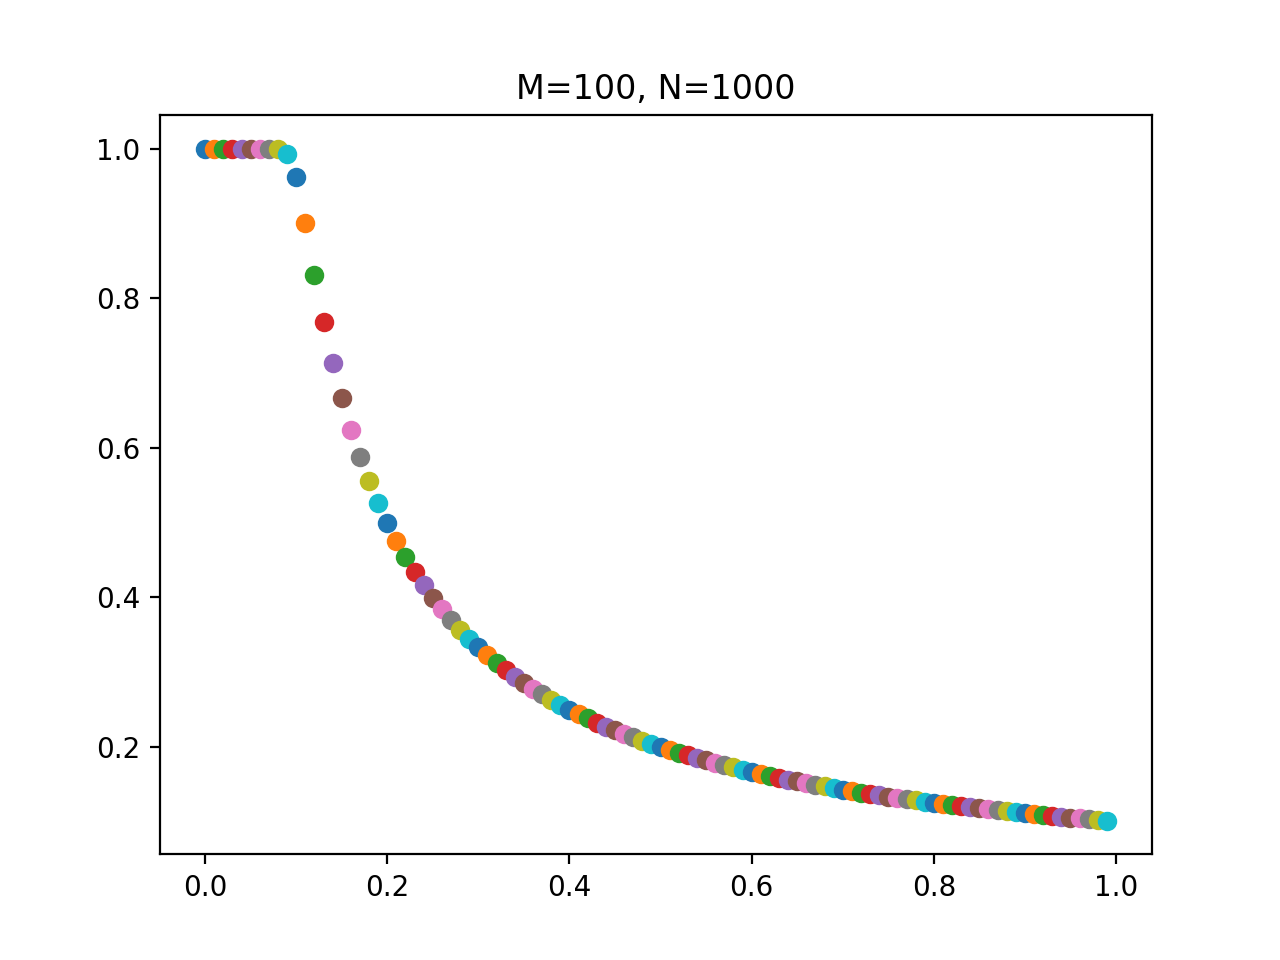
\includegraphics[scale=.6]{img/1000_100}
\end{frame}

%------------------------------------------------

\begin{frame}
\frametitle{Основная литература}
\nocite{gas}
\nocite{rough2005}
\nocite{agt2007}
\printbibliography[heading=bibintoc]
\end{frame}

%------------------------------------------------

\begin{frame}
\Huge{\centerline{Спасибо за внимание!}}
\end{frame}

%----------------------------------------------------------------------------------------

\end{document} 
